\documentclass[a4paper,12pt]{article}

\usepackage{geometry}
\usepackage{cmap}
\usepackage{enumerate}
\usepackage[russian]{babel}
\usepackage{hyperref}
\usepackage{listings}
\usepackage{verbatim}
\usepackage{pdfpages}
\usepackage[font=small,labelfont=bf]{caption}
\usepackage{float} 

\geometry{a4paper, left=20mm, right=10mm, top=20mm, bottom=20mm}

\lstdefinestyle{cppcode}{
	basicstyle=\ttfamily
}

\lstset{language=C++,style=cppcode}

\begin{document}

\begin{titlepage}		

\begin{center}
	\textsc{\textbf{Правительство Российской Федерации}}\\
	\vspace{0.5cm}
	\hrule
	\vspace{0.5cm}
	\textsc{Федеральное государственное автономное образовательное учреждение высшего образования <<Национальный исследовательский университет <<Высшая школа экономики>>}\\
	\vspace{1cm}
	Кафедра <<Компьютерная безопасность>>
\end{center}	

\vspace{\fill}

\begin{center}
	\Large{\textbf{ОТЧЕТ \\ К ЛАБОРАТОРНОЙ РАБОТЕ №3}} \\
	\vspace{1em}
	\textbf{по дисциплине} \\
	\vspace{1em}
	\large{\textbf{<<Языки программирования>>}}
\end{center}

\vspace{\fill}

\begin{flushright}
	\begin{minipage}[center]{15cm}
		\begin{minipage}[left]{5cm}
			{Работу выполнил\\студент группы СКБ-203}
		\end{minipage}
		\begin{minipage}[center]{5cm}
			\vspace{1.25cm}
			\hrulefill\\[-1cm]
			\begin{center}{подпись, дата}\end{center}
		\end{minipage}
		\begin{minipage}[right]{4cm}
			\vspace{0.4cm}
			\begin{flushright}{К.А. Павкин}\end{flushright}
		\end{minipage}
		\\
		\\
		\\
		\begin{minipage}[left]{5cm}
			{Работу проверил}
		\end{minipage}
		\begin{minipage}[center]{5cm}
			\vspace{1.25cm}
			\hrulefill\\[-1cm]
			\begin{center}{подпись, дата}\end{center}
		\end{minipage}
		\begin{minipage}[right]{4cm}
			\begin{flushright}{С.А. Булгаков}\end{flushright}
		\end{minipage}
	\end{minipage}
\end{flushright}

\vspace{\fill}

\begin{center}
	Москва~2021
\end{center}

\end{titlepage}

\tableofcontents
\thispagestyle{empty}
\cleardoublepage

\section*{<<Итератор>>}\addcontentsline{toc}{section}{Постановка задачи}

Разработать программу на языке Си++ (ISO/IEC 14882:2014), демонстрирующую решение поставленной задачи.
Весь код разбить на заголовочные файлы *.h и соответствующие им файлы реализации *.cpp (а также main.cpp, файл конфигурации системы сборки CMake и отчет о покрытии кода).
По выполненной работе составить отчет согласно требованиям ГОСТ 7.32-2017, содержащий диаграмму классов согласно спецификации UML 2.0 и предоставить его копию в формате PDF.
Все необходимые файлы разместить в git-репозитории (ссылка будет указана отдельно), взаимодействие выполнять с использованием платформы GitHub.
Решения, предоставленные иными способами, не принимаются.
Выполненные работы подлежат процедуре защиты.
Необходимым условием является защита лабораторной работы 2.
Защита проводится во время срока выполнения работы.
Срок выполнения работы 19 июня 2021 года.
После истечения срока работа считается не сданной и оценивается в 0 баллов.
Все присланные работы проверяются на отсутствие ошибок сборки в автоматическом режиме, в случае отсутствия ошибок выполняется ручная проверка кода, в противном случае работа оценивается в 0 баллов.
Ручная проверка работ выполняется преподавателем – оценивается полнота выполнения задания, а также качество решения.
Оценка выставляется в 10 балльной шкале.
Все работы проверяются в системе Антиплагиат.
Компилятор и операционная система, используемые при проверке: GNU Compiler Collection 10.2.0 цель x86\_64-slackware-linux система Slackware Linux current 2020-10-26.

\subsection*{Постановка задачи}

Переработать классы, разработанные в рамках лабораторной работы 2.


Разработать шаблоны классов, объекты которых реализуют типы данных, указанные ниже. Для этих шаблонов классов разработать необходимые конструкторы, деструктор, конструктор копирования.
Разработать операции: добавления/удаления элемента (уточнено в задаче); получения коли- чества элементов; доступа к элементу (перегрузить оператор []). При ошибках запускать исключение.

Разработать два вида итераторов (обычный и константный) для указанных шаблонов классов.

В главной функции разместить тесты, разработанные с использованием библиотеки GoogleTest.

При разработке тестов, добиться полного покрытия.
Отчет о покрытии приложить к работе.

\subsubsection*{Задачи}

\begin{enumerate}
	
\item
Шаблон «динамический массив объектов».
Размерность массива не изменяется в момент его переполнения.
Начальная размерность задается как параметр конструктора, значение по умолчанию 0.
Метод изменения размера.
Добавление/удаление элемента в произвольное место.

\item
Шаблон «стек» (внутреннее представление – динамический массив хранимых объектов).
Размерность стека увеличивается в момент его переполнения.
Начальная размерность задается как параметр конструктора, значение по умолчанию 0.
Добавление/удаление элемента в начало и в конец.

\item
Шаблон «односвязный список объектов».
Добавление/удаление элемента в произвольное место.

\item
Шаблон «циклическая очередь» (внутреннее представление – динамический массив хранимых объектов).
Добавление/удаление элемента в произвольное место.

\item
Шаблон «двоичное дерево объектов».
Добавление/удаление элемента в произвольное место.

\end{enumerate}

\cleardoublepage

\section{Алгоритм решения задачи}

В процессе анализа предметной области были выявлены основные алгоритмы, необходимые для реализации всеобъемлющей, асимптотически эффективной и отлаженной программы для решения поставленной задачи.

На рисунке \ref{Class} представлена диаграмма классов, демонстрирующая формат хранения данных и зависимости между классами.
В целях сужения диаграммы без ущерба логике и смыслу были опущены закрытые служебные методы.

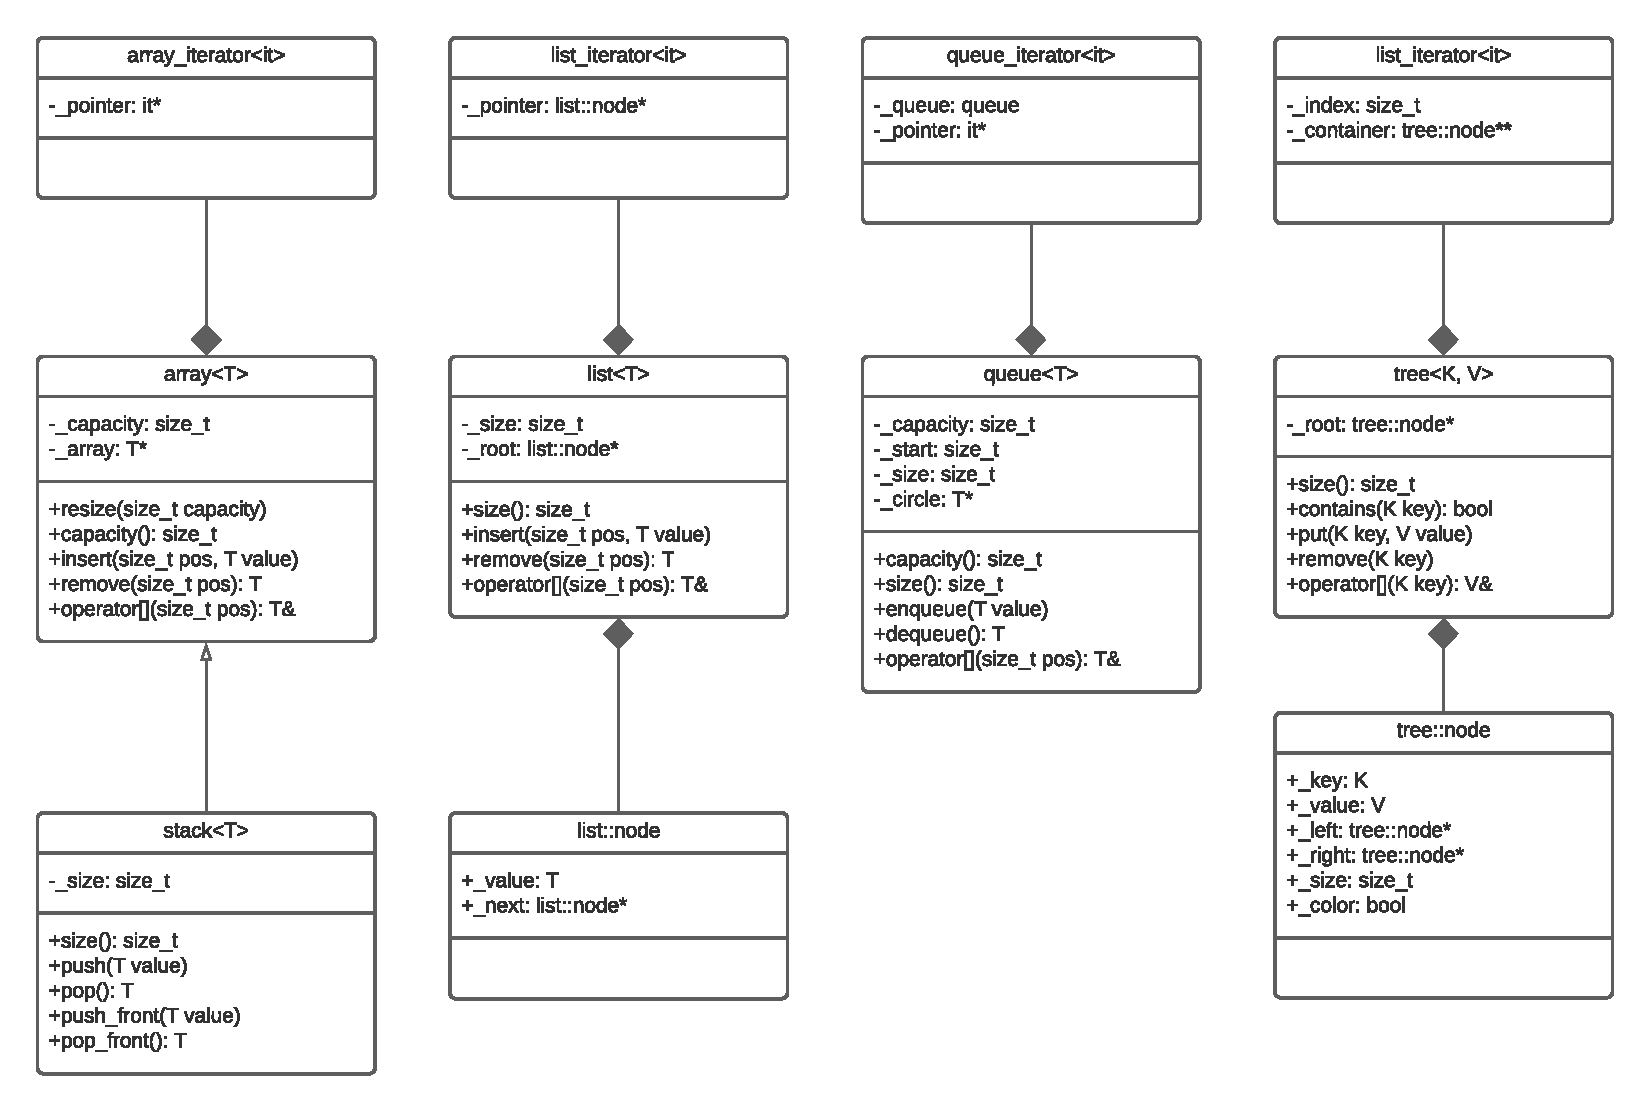
\includegraphics[width=\textwidth]{UML Class.pdf}

\captionof{figure}{Диаграмма классов}\label{Class}

\cleardoublepage

\subsection{Динамический массив}

Итератор для динамического массива предельно простой, поскольку внутри такой контейнер представлен как непрерывная последовательность ячеек памяти.
Таким образом, для итерации по динамическому массиву достаточно воспользоваться стандартной арифметикой указателей.

В связи с некоторыми отличиями текущего задания от предыдущего, класс для представления контейнера был несколько переработан.
В частности, процедура resize была вынесена к публичным методам, и операции вставки/удаления больше не инициируют изменение размерности. За ненадобностью была удалена переменная size, ранее необходимая для хранения количества заполненных элементов динамического массива.

Полный код заголовочных файлов и файлов реализации динамического массива приведены в приложении А.

\subsubsection{Стек}

Стек, будучи наследуюемым от динамического массива, не имеет отличий при работе с итератором.

Однако, требования для стека отличаются от требований для динамического массива. Теперь стек содержит переменную size, а также инициирует изменение размерности контейнера в случаях его сужения/переполнения.

Полный код заголовочных файлов и файлов реализации стека приведены в приложении Б.

\cleardoublepage

\subsection{Односвязный список}

В отличие от динамического массива, элементы односвязного списока не представлены в виде непрерывной последовательности ячеек в памяти.
Для итерирования по контейнеру необходимо передавать указатель на \verb!node! и при увеличении итератора заполнять его значение следующим — \verb!node = node->next!. Концом контейнера считается значение \verb!nullptr!, что является корректным решением, поскольку ни один заполненный узел, даже имея пустое значенение, не обращается в пустой указатель.

Полный код заголовочных файлов и файлов реализации односвязного списка приведены в приложении В.

\cleardoublepage

\subsection{Циклическая очередь}

Хотя по представлению элементов в памяти циклическая очередь схожа с динамическим массивом, она имеет такую особенность, что указатель на конец контейнера может находиться в памяти левее, чем указатеель на его начало.
Поэтому было решено дополнительно передавать в итератор указатель на очередь. При достижении итератором конца контейнера, значение указателя сбрасывается до начала очереди.

Полный код заголовочных файлов и файлов реализации односвязного списка приведены в приложении Г.

\cleardoublepage

\subsection{Бинарное дерево}

Бинарное дерево является самым нетривиальным для итерирования контейнером.
Дело в том, что при итерации существует необходимость сохранять порядок элементов, а стандартный поиск в ширину не удовлетворяет данному условию, поскольку в текущей реализации дерева в левых потомках содержатся только меньшие ключи, а в правых — только большие.
Поиск в глубину тоже не решает задачу, ибо в текущей реализации бинарного дерева не хранятся указатели на родительский узел, а адаптация существующего интерфейса под нужды итератора — это кощунство по отношению к уже реализованным модулям.

Таким образом, было решено передавать в итератор указатель на корневой узел (точно так же, как это сделано в односвязном списке), и в конструкторе единожды заполнять временный контейнер, представленный динамическим массивом, с помощью поиска в глубину.
Для поддержания указателя на конец дерева, размерность временного контейнера на единицу превышает количество элементов дерева, и последний элемент заполнен значением \verb!nullptr!.
Аналогично односвязному списку, значение \verb!node! обращается в пустой указатель только в том случае, если был достигнут конец контейнера.

Функция \verb!fill_container!, заполняющая временный контейнер исходя из значения указателя на корневой узел, представлена в листинге \ref{lst1}.

\begin{lstlisting}[caption={Функция для заполнения временного контейнера},label=lst1]
size_t fill_container(node* pointer, size_t index)
{
	if (pointer == nullptr) {
		return index;
	}
	
	index = fill_container(pointer->_left, index);
	
	_container[index] = pointer;
	
	return fill_container(pointer->_right, index + 1);
}
\end{lstlisting}

Полный код заголовочных файлов и файлов реализации бинарного дерева приведены в приложении Д.

\cleardoublepage

\section{Получение исполняемых модулей}

Заголовочные файлы и их реализации были размещены в различных директориях.
Для сборки проекта в каждую директорию были помещены файлы CMakeLists.txt, и, таким образом, каждая директория представляет из себя отдельную библиотеку, которая в последствии собирается в корневом каталоге.
Файл сборки CMakeLists.txt из корневого каталога показан в листинге \ref{CMakeLists}.

\begin{lstlisting}[caption={Файл сборки CMakeLists.txt},label=CMakeLists]
cmake_minimum_required(VERSION 3.0)

project(laboratory-work-03-kapavkin)

set(CMAKE_CXX_STANDARD 14)
set(CMAKE_CXX_FLAGS --coverage)

include(FetchContent)
FetchContent_Declare(
googletest
URL https://github.com/google/googletest/archive/609281088cfefc76f9d0
ce82e1ff6c30cc3591e5.zip
)

set(gtest_force_shared_crt ON CACHE BOOL "" FORCE)
FetchContent_MakeAvailable(googletest)

set(MAIN main.cpp)

enable_testing()

add_executable(main ${MAIN})

add_subdirectory(array)
add_subdirectory(list)
add_subdirectory(queue)
add_subdirectory(tree)

target_link_libraries(main
array
list
queue
tree
gtest_main
)

include(GoogleTest)
gtest_discover_tests(main)
\end{lstlisting}

\cleardoublepage

\section{Тестирование}

В целях проверки корректности работы реализованных классов были проведены процедуры тестирования приложения, разработаны тест-кейсы с использованием библиотеки \verb!Google Test!, составлен отчет о покрытии кода с помощью утилиты \verb!gcov!.

\subsection{Варианты использования}

Файл main.cpp! содержит юнит-тесты, целью которых является сравнение ожидаемых от функций значений с фактическими, и выдача оповещений при их несовпадении.

\subsubsection{Класс {\tt array}}

Тестовые случаи для проверки корректности работы методов класса {\tt array}.

\begin{enumerate}

\item
\verb!constructor! — проверяет корректность конструкторов/деструкторов.

\item
\verb!insert! — проверяет корректность вставки элемента в произвольное место.

\item
\verb!remove! — проверяет корректность удаления элемента из произвольного места.

\item
\verb!iterator! — проверяет корректность итерирования по динамическому массиву и совпадение полученного в результате итерирования количества элементов с размером контейнера.

\end{enumerate}

\subsubsection{Класс {\tt stack}}

Тестовые случаи для проверки корректности работы методов класса {\tt stack}.

\begin{enumerate}

\item
\verb!constructor! — проверяет корректность конструкторов/деструкторов.

\item
\verb!push! — проверяет корректность вставки элемента в конец стека.

\item
\verb!pop! — проверяет корректность удаления элемента из конца стека.

\item
\verb!iterator! — проверяет корректность итерирования постеку и совпадение полученного в результате итерирования количества элементов с размером контейнера.

\end{enumerate}

\subsubsection{Класс {\tt list}}

Тестовые случаи для проверки корректности работы методов класса {\tt list}.

\begin{enumerate}

\item
\verb!constructor! — проверяет корректность конструкторов/деструкторов.

\item
\verb!insert! — проверяет корректность вставки элемента в произвольное место.

\item
\verb!remove! — проверяет корректность удаления элемента из произвольного места.

\item
\verb!iterator! — проверяет корректность итерирования по односвязному списку и совпадение полученного в результате итерирования количества элементов с размером контейнера.

\end{enumerate}

\subsubsection{Класс {\tt queue}}

Тестовые случаи для проверки корректности работы методов класса {\tt queue}.

\begin{enumerate}

\item
\verb!constructor! — проверяет корректность конструкторов/деструкторов.

\item
\verb!enqueue! — проверяет корректность вставки элемента в конец очереди.

\item
\verb!dequeue! — проверяет корректность удаления элемента из начала очереди.

\item
\verb!oversize! — проверяет корректность при переполнении очереди.

\item
\verb!iterator! — проверяет корректность итерирования по циклической очереди и совпадение полученного в результате итерирования количества элементов с размером контейнера.

\end{enumerate}

\subsubsection{Класс {\tt tree}}

Тестовые случаи для проверки корректности работы методов класса {\tt tree}.

\begin{enumerate}
	
\item
\verb!constructor! — проверяет корректность конструкторов/деструкторов.

\item
\verb!put! — проверяет корректность вставки элемента в произвольное место.

\item
\verb!remove! — проверяет корректность удаления элемента из произвольного места.

\item
\verb!iterator! — проверяет корректность итерирования по красно-черному дереву и совпадение полученного в результате итерирования количества элементов с размером контейнера.

\end{enumerate}

\subsection{Отчет о покрытии кода}

На рисунке \ref{Coverage} показан отчет о покрытии кода тестами.

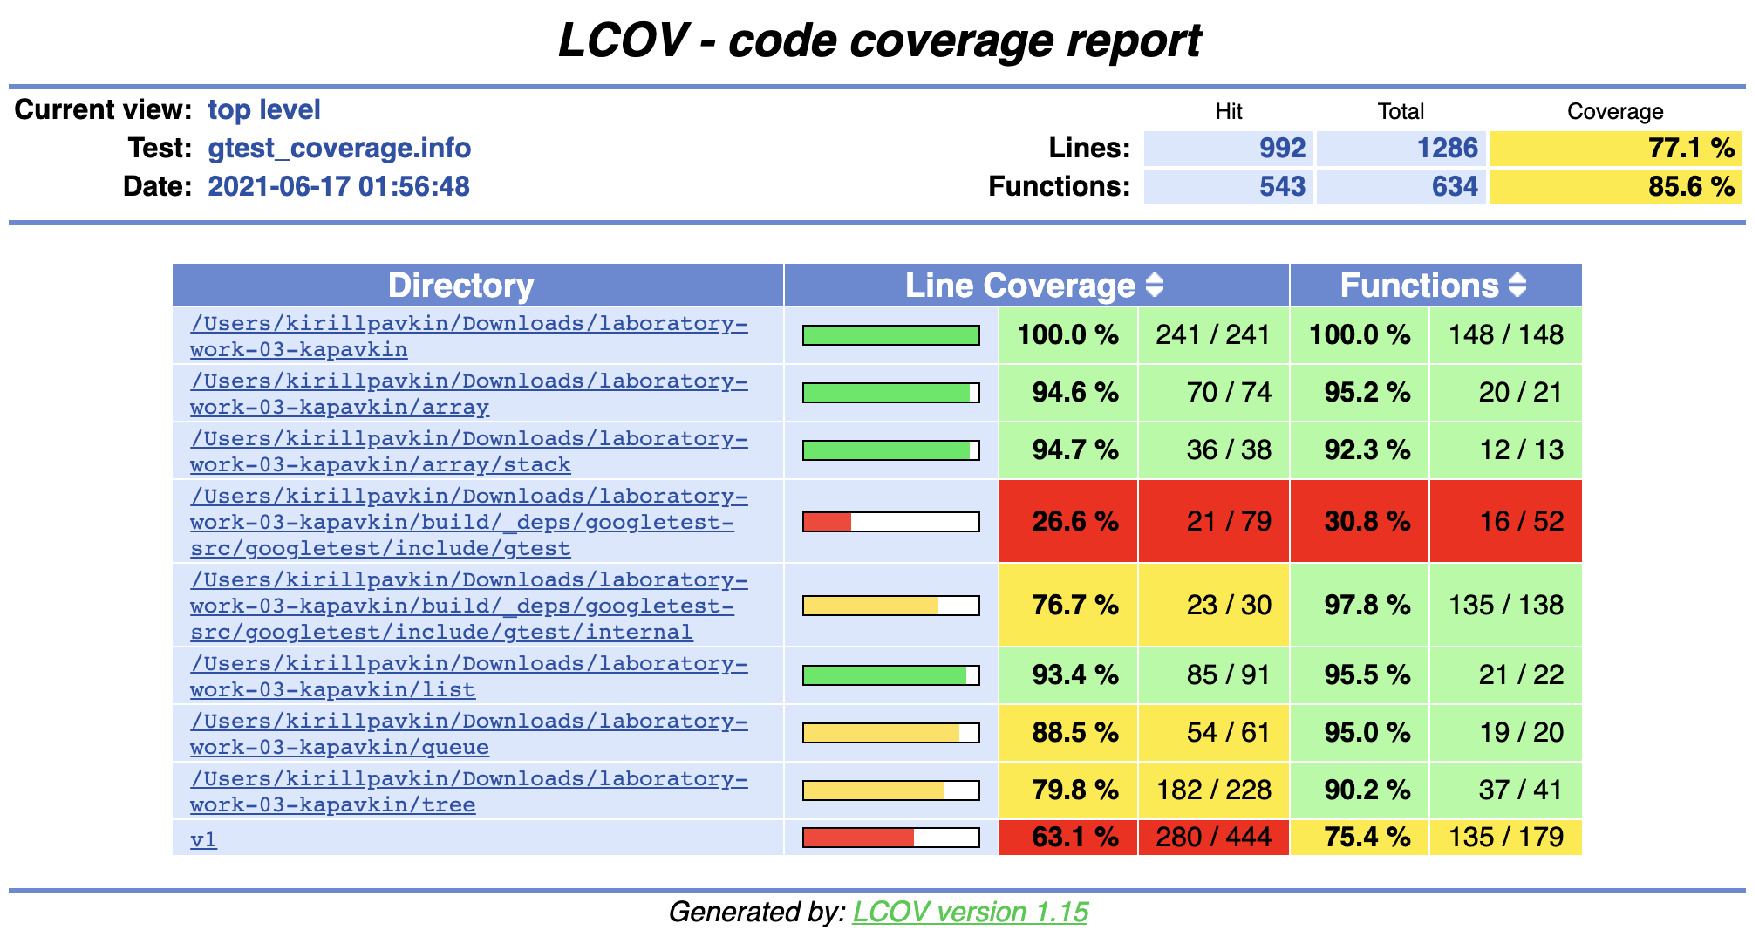
\includegraphics[width=\textwidth]{Coverage.pdf}

\captionof{figure}{Отчет о покрытии кода}\label{Coverage}

\cleardoublepage

\section*{\begin{center} Приложение А \end{center}}\label{AA}\addcontentsline{toc}{section}{Приложение А}

\subsection*{А.1 Заголовочный файл класса array}\label{AA1}

\verbatiminput{../array/array.h}

\subsection*{А.2 Файл реализации класса array}\label{AA2}

\verbatiminput{../array/array.cpp}
\cleardoublepage

\section*{\begin{center} Приложение Б \end{center}}\label{AB}\label{AA}\addcontentsline{toc}{section}{Приложение Б}

\subsection*{Б.1 Заголовочный файл класса stack}\label{AB1}

\verbatiminput{../array/stack/stack.h}

\subsection*{Б.2 Файл реализации класса stack}\label{AB2}

\verbatiminput{../array/stack/stack.cpp}
\cleardoublepage

\section*{\begin{center} Приложение В \end{center}}\label{AC}\label{AA}\addcontentsline{toc}{section}{Приложение В}

\subsection*{В.1 Заголовочный файл класса list}\label{AC1}

\verbatiminput{../list/list.h}

\subsection*{В.2 Файл реализации класса list}\label{AC2}

\verbatiminput{../list/list.cpp}
\cleardoublepage

\section*{\begin{center} Приложение Г \end{center}}\label{AD}\label{AA}\addcontentsline{toc}{section}{Приложение Г}

\subsection*{Г.1 Заголовочный файл класса queue}\label{AD1}

\verbatiminput{../queue/queue.h}

\subsection*{Г.2 Файл реализации класса queue}\label{AD2}

\verbatiminput{../queue/queue.cpp}
\cleardoublepage

\section*{\begin{center} Приложение Д \end{center}}\label{AE}\label{AA}\addcontentsline{toc}{section}{Приложение Д}

\subsection*{Д.1 Заголовочный файл класса tree}\label{AE1}

\verbatiminput{../tree/tree.h}

\subsection*{Д.2 Файл реализации класса tree}\label{AE2}

\verbatiminput{../tree/tree.cpp}
\cleardoublepage

\end{document}